\documentclass[11pt]{article}
\usepackage{geometry}
\usepackage{graphicx}
\usepackage{wrapfig}
\usepackage{float}
\usepackage[T1]{fontenc}
\usepackage[utf8]{inputenc}
\usepackage{helvet}
\renewcommand{\familydefault}{\sfdefault}
\usepackage{titlesec}
\titlespacing\section{1pt}{12pt plus 2pt minus 2pt}{1pt plus 2pt minus 2pt}
\titlespacing\subsection{1pt}{12pt plus 2pt minus 2pt}{pt plus 2pt minus 2pt}
%\titlespacing\subsubsection{5pt}{12pt plus 2pt minus 2pt}{1pt plus 2pt minus 2pt}
%\usepackage{float}
\usepackage[hidelinks]{hyperref}
\geometry{margin=0.5in}
%opening
\titleformat*{\section}{\small\bfseries}
\title{Investigating the genetic diversity, population structure and demography of Baja and Pacific \emph{Odontodactylus scyllarus}}
\bibliographystyle{unsrt}
\date{}
\author{Ethan Holleman}
\begin{document}
\maketitle
\thispagestyle{empty}

\section{Background}

\emph{Odontodactylus scyllarus}, or the Mantis shrimp are a unique group of carnivorous stomatopods that are believed to have diverged from the class Malacostraca around 340 million years ago \cite{VanDerWal2017}. Mantis shrimp are notable for both their unique mechanically driven raptorial smashing claws which are powerful enough to induce cavitation in the surrounding water \cite{Patek2004, Patek2005} and acutely sensitive visual system which is believed to be the most complex ever discovered in nature \cite{Cronin2014, Milius2012}. Due to their extraordinary physiology the biology of Mantis shrimp species has been the subject of significant study but comparatively few studies have focused on the genetic structure of Mantis shrimp populations and have focused on Asian Mantis shrimp species in the Yellow and East China Seas \cite{Yang2018}. Mantis shrimp are known to play an important role in marine ecosystems by acting as efficient predators of other crustaceans and oxygenating ocean sediments \cite{Antony2010}. 


\begin{wrapfigure}{l}{0.35\textwidth}
	\begin{center}
		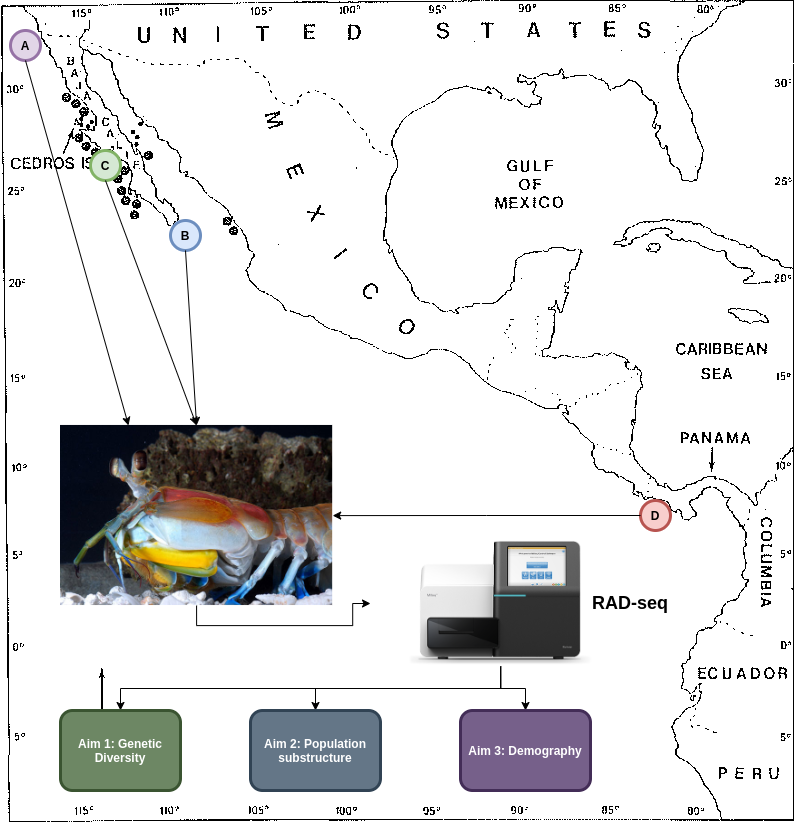
\includegraphics[width=0.30\textwidth]{images/sampling_locations.png}
	\end{center}
	\caption{Proposed \emph{Hemisquilla californiensis} collection locations shown as colored dots. Image adapted from \emph{Basch et al, 93}}
\end{wrapfigure}

Main goal is to resolve the genetic diversity of \emph{Hemisquilla californiensis} ranges from Santa Barba California to Bay of Panama 
population mapping efforts preceded the advent of next-generation sequencing technologies

In this effort we will pursue three specific aims. 


\section*{Aim 1: Quantify genetic variation of the California Mantis shrimp}
Hypothesis: \emph{Odontodactylus scyllarus} will show significant genetic variation between sampling locations.

Locations,   number   of   samples   (N),   percent amplification  (%A),  useable  samples  (N*),  mean  allelicrichness   (AR),   expected   heterozygosity   (He),   observedheterozygosity   (Ho),   and   inbreeding   F-statistics   (FIS)based  on  16  microsatellite  loci  for  35  populations  ofO.mykissfrom the Klamath–Trinity River basin



Use double-digest restriction site associated DNA sequencing (RAD-seq) \cite{Peterson2012}. Challenge will be the lack of reference genome for shrimp as non-model organism. Also utilize the a total mitochondrial genome of \emph{Squilloides leptosquilla} \cite{Kang2015}, a mantis shrimp species closely related to \emph{Odontodactylus scyllarus}. 

Will rely on the closely related \emph{Litopenaeus vannamei},  Pacific white shrimp, genome \cite{Zhang2019}


\section*{Aim 2: Evaluate sub-population structure within sampling locations}
Mantis shrimp species are known to be mostly solitary creatures, rarely spending significant amounts of time outside of their sea floor burrows \cite{Mead2010}. This small range is expected to give rise to significant population sub-structure within the four sampling locations. 


\begin{itemize}
	\item Fixation Index: reduction in genetic diversity of sub populations due to differentiation among sub populations.
	\begin{itemize}
		\item Access the reduction of differentiation to compare specific sub-populations using pairwise comparison. 
		\item How to define different sub populations? Blobs of areas / habitats
		\item High pairwise Fst to gauge the distinctness of populations. Do something where defining subpopulations 
		at greater and greater distances to determine how quickly Fst will drop off at different sampling sites. 
	\end{itemize}
	\item Another entry in the list
\end{itemize}



Expected heterozygotes Ht (total population was randomly mating)
Collect genotype data from a single locus A/T SNP and collect
adults 
Determine allele frequencies of locus interested in
This is where would look at mean Fst (fixation index which is mean reduction in Hs (expected heterozygotes due to genetic differentiation among sub-populations)).
Fis (inbreeding coefficient reduction in Hi due to non-random mating within a sub-populations )
Bayesian sub-population assignment 
possibly admixture analysis here as well


\section*{Aim 3: Determine demographic history of two sub-populations of these bugs}

Hypothesis recent decline in mantis schrimp that coinsides with
human activity. Mantis schrimp are sensitive to oceanic changes that effect them directly and habitat. 

Evaluate the effect of selection on the observed site frequency spectrum gleaned from RAD-seq data collected as a part of aim 1 by evluating the allele frequency selection of each suitable locus compared to the allele frequency spectrum of all other suitable loci across the genome. 

Would expect this to be demographic event though since fast maybe too extreme? This article suggests that 

Ocean acidification would not effect mantis shrimp because did not really affect their weapons
https://www.nature.com/articles/srep38637

\begin{itemize}
	\item How to tell demography vs selection?
	\begin{itemize}
		\item Wright-Fisher model predicts something. Neutral expectation. Constant size and no selection.
		\item Selection
		\begin{itemize}
			\item Selective sweep
			\item negative selection
			\item balancing selection 
			\item Any of these is occurring at specific loci that is under selection compared to a population (demographic level) change that should be observed genome wide because not specific to specific locus. 
		\end{itemize}
		\item Historical demography of a population
		\begin{itemize}
			\item Step 1 determine allele frequency spectrum of a population by sampling individuals and determine what that is 
			\item Neutral site freq spectrum has predictable decay but when looking at actual population and determine allele freq spectrum which might differ greatly from neutral expectation
			\item Step 2 is build some demographic model
			\begin{itemize}
				\item Pop size on y and time on x axis
				\item Shows how population size has changed over time
				\item s is the strength of the decline (or more generally the change in population size)
			\end{itemize}
			\item Step 3 Determine the parameters that we are going to vary
			\begin{itemize}
				\item Might want to determine the
					\item Strength of decline
					\item Timing of decline
					\item Rate of expansion
					\item Some combination
					\item These are the things that we are trying to determine. 
			\end{itemize}
			\item Step 4: Simulate data with different model parameter values.
			\begin{itemize}
				\item Get a simulated SFS sSFS
				\item DO many many simulations where you change the variables of interest and compare simulated SFS to observed SFS to try and find the parameter valeus that produce a simulated SFS to the population we are interested in.
				\item This is ABC approximate Bayesian computation
				\item Requires defining a prior distribution that will define the parameter space
				\item Simulate with the same amount of data that
				we collected and get gene copies sequences (simulated) which allows for calculating the
				simulated allele frequency spectrum 
				 
			\end{itemize}
		\end{itemize}
	\end{itemize}
\end{itemize}

5038141913


\pagebreak

\bibliography{refs}

\end{document}
